\documentclass[12pt]{article}
%%%%%%%%%%%%%%%%%%%%%%%%%%%%%
% Preambulo
%
\usepackage[T1]{fontenc}
\usepackage[utf8]{inputenc}
\usepackage[spanish]{babel}
\parindent=0cm %modificar tamaño de sangria 
\usepackage{amsmath}
\usepackage{amssymb,amsfonts,latexsym,cancel}
%
\usepackage{graphicx}
\usepackage{epstopdf}
\usepackage{float}
\usepackage{subfigure}
%%%%%%%%%%%%%%%%%%%%%%%%%%%%%
\begin{document}
\title{Practica 4.\\ Gráficas}
\author{Héctor Misael}
\date{}
\maketitle
\tableofcontents

\section{Incluir gráficas externas}
En \LaTeX podemos incluir figuras externas o generadas  directamente en \LaTeX \, utilizando algún paquete, algunos de los formatos que podemos utilizar son \textbf{.jpg}, \textbf{.png}, \textbf{.eps} y \textbf{.pdf}.\\[0.5cm]
Los formatos vectoriales como los son \textbf{.eps} y \textbf{.pdf} son los mas recomendados cuando hacemos gráficas en las cuales queremos observar detalles y precisión, porque no pierden calidad al aumentar o disminuir su tamaño. y para imágenes en general podemos utilizar los formatos \textbf{.jpg} o \textbf{.png}

\subsection{Paquete graphicx}
\begin{center}
\includegraphics[scale=0.4]{figuras/imagen1.pdf}
\end{center}

\begin{itemize}
\item scale: Escala de la imagen
\item width: Ancho deseado de la imagen en cm.
\item height: Altura deseada de la imagen en cm.
\end{itemize}

\begin{center}
\includegraphics[scale=0.1]{figuras/imagen1.pdf}
\end{center}

\begin{center}
\includegraphics[width=4cm]{figuras/imagen1.pdf}
\end{center}

\begin{center}
\includegraphics[height=5cm]{figuras/imagen1.pdf}
\end{center}

\begin{center}
\includegraphics[scale=0.1]{figuras/imagen1.pdf} \quad
\includegraphics[scale=0.2]{figuras/imagen1.pdf} \quad
\includegraphics[scale=0.3]{figuras/imagen1.pdf} \quad
\includegraphics[scale=0.4]{figuras/imagen1.pdf} 
\end{center}

%\newpage
\section{Objetos flotantes}
En \LaTeX podemos incluir figuras externas o generadas  directamente en \LaTeX \, utilizando algún paquete, algunos de los formatos que podemos utilizar son \textbf{.jpg}, \textbf{.png}, \textbf{.eps} y \textbf{.pdf}.

\begin{figure}[!ht]
\centering
\includegraphics[scale=0.5]{figuras/imagenmat.pdf}
\put(-270,110){\footnotesize{usando el comando put}}
\put(-270,90){$x+1$}
\caption{imagen a escala 0.5}
\label{figura1}
\end{figure}

Los formatos vectoriales como los son \textbf{.eps} y \textbf{.pdf} son los mas recomendados cuando hacemos gráficas en las cuales queremos observar detalles y precisión, porque no pierden calidad al aumentar o disminuir su tamaño. y para imágenes en general podemos utilizar los formatos \textbf{.jpg} o \textbf{.png}

\begin{itemize}
\item t: La imagen en la parte superior (top)
\item b: La imagen en la parte inferior (bottom)
\item h: La imagen en el sitio que escribimos (here)
\end{itemize}

\begin{figure}[H]
\centering
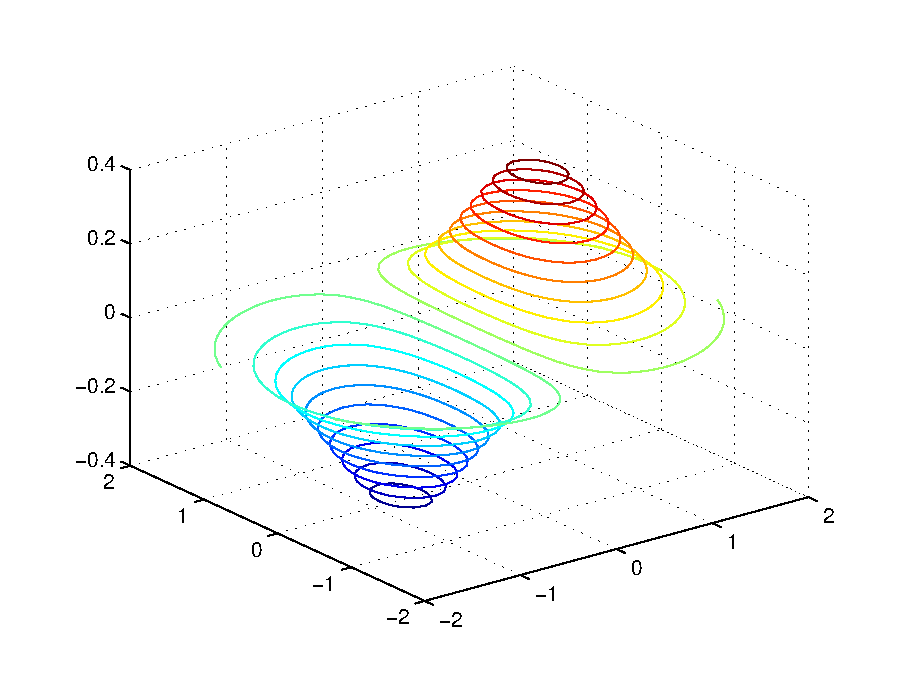
\includegraphics[scale=0.5]{figuras/imagenmat2.eps}
\caption{imagen con formato eps}
\label{figura1}
\end{figure}

\subsection{Paquete float}

\begin{figure}[H]
\centering
\includegraphics[scale=0.3]{figuras/elefante}
\caption{imagen con formato jpg}
\label{figura2}
\end{figure}

Como lo muestra la imagen \eqref{figura2}.\\
En \LaTeX podemos incluir figuras externas o generadas  directamente en \LaTeX \, utilizando algún paquete, algunos de los formatos que podemos utilizar son \textbf{.jpg}, \textbf{.png}, \textbf{.eps} y \textbf{.pdf}.\\[0.5cm]
Los formatos vectoriales como los son \textbf{.eps} y \textbf{.pdf} son los mas recomendados cuando hacemos gráficas en las cuales queremos observar detalles y precisión, porque no pierden calidad al aumentar o disminuir su tamaño. y para imágenes en general podemos utilizar los formatos \textbf{.jpg} o \textbf{.png}

\begin{figure}[H]
\centering
\includegraphics[scale=0.15]{figuras/Petirrojo2}
\caption{imagen con formato jpg}
\label{figura3}
\end{figure}

\newpage
\subsection{Paquete subfigure}

\begin{figure}[!ht]
\centering
\subfigure[Primera figura]
{\includegraphics[scale=0.1]{figuras/Petirrojo2}}
\quad
\subfigure[Segunda figura]
{\includegraphics[scale=0.1]{figuras/Petirrojo2}}
\quad
\subfigure[Tercera figura]
{\includegraphics[scale=0.1]{figuras/Petirrojo2}}
\caption{varias figuras con subfigure}
\label{figurasvarias}
\end{figure}

Tal como aparece en la figura anterior \eqref{figurasvarias}.

\end{document}